\documentclass[10pt]{article}

\usepackage{spheric}
%%%TITLE
\title{The Hermit-type RRKPM for piezoelectric materials}
\date{}

%%AFFILIATIONS
\author[$\relax$]{Jichao MA}
\author[$\relax$]{Gaofeng WEI$^\dagger$}
\affil[$\relax$]{Qilu University of Technology, China}
\affil[$\relax$]{\email{\dagger}{wgf@spu.edu.cn}}


%%DOCUMENT
\begin{document}

\maketitle

%\SelectedTopics{}

%%PLEASE PUT YOUR ABSTRACT HERE
\begin{abstract}
In this paper, the radial basis function (RBF) and its normal derivative are introduced into the reproducing kernel particle method (RKPM), and the Hermit-type radial reproducing kernel particle method (Hermit-type RRKPM) is proposed. The method can reduce the adverse effect of the kernel function on the calculation precision. The errors can be decreased on the boundary, and the accuracy and stability of the method are improved. Then the proposed method is applied to the numerical simulation of piezoelectric materials. The numerical results show that the Hermit-type RRKPM is more stable and accurate than the RKPM.

Take a piezoelectric strip as the example to analyze the bending deformation. It is subjected to a linear stress in the $x$-direction and an applied voltage in the $z$-direction. (i) Analytical solutions and numerical solutions are analyzed in the $x$-direction. (ii) Analytical solutions and numerical solutions are analyzed in the $z$-direction. The results are pretty close.


\begin{figure}[!htb]
\centering
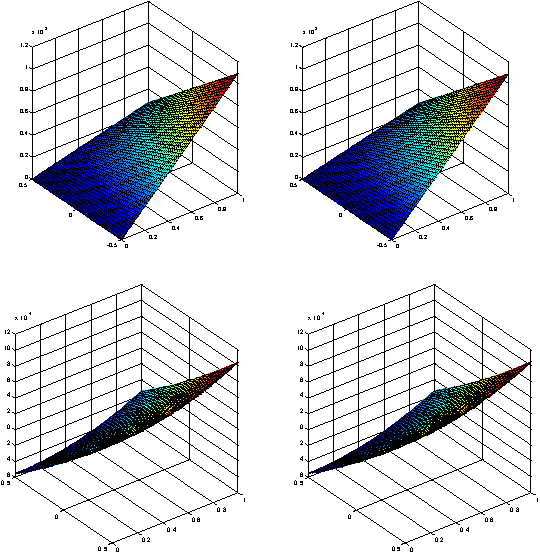
\includegraphics[width=0.7\textwidth]{23-1.pdf}
\caption{The comparison between the analytical solutions and numerical solutions}\label{fig:23}
\end{figure}

\end{abstract}


%%THE END OF ABSTRACT

\addbib

\end{document}
